%\documentclass[12pt,PhD,twoside]{muthesis}
%\usepackage{verbatim}
%\usepackage{graphicx}
%\graphicspath{ {img/} }
%\usepackage{url} % typeset URL's reasonably
%\usepackage{listings}
%\usepackage{pdfpages}
%\usepackage{tabu}
%\usepackage{longtable}
%\usepackage{multirow, tabularx}
%\usepackage[labelfont=bf]{caption}
%\usepackage{natbib}
%\usepackage{pslatex} % Use Postscript fonts
%\usepackage{amsmath}
%\usepackage{amssymb}
%\usepackage{bm}
%\usepackage{pseudocode}
%\DeclareMathOperator*{\argmin}{arg\,min}
%\DeclareMathOperator*{\argmax}{arg\,max}
%\def\approxprop{%
%	\def\p{%
%		\setbox0=\vbox{\hbox{$\propto$}}%
%		\ht0=0.6ex \box0 }%
%	\def\s{%
%		\vbox{\hbox{$\sim$}}%
%	}%
%	\mathrel{\raisebox{0.7ex}{%
%			\mbox{$\underset{\s}{\p}$}%
%		}}%
%	}
%\begin{document}
%\bibliographystyle{model5-names}

%\chapter[Probabilistic neural models and their plausibility]{Neural implementations of uncertainty and inference and their consistency with the hippocampal complex}

\chapter{Supplementary Information for Chapter 6: Towards real-world capable spatial memory in the LIDA cognitive architecture}
\label{apx:lidaspm}
\section{Comparison of hierarchical activation gradient-based route planning with human performance on the TSP task}


In order to evaluate the plausibility of gradient-based multi-goal route planning, as described in the main text (see Figure 5), we have used data collected from participants recruited on Amazon Mechanical Turk, tasked with solving the travelling salesperson problem (TSP) in virtual reality environments. Data from 46 participants was analysed here. They were asked to mark all buildings in the 3D environment and then return to the building they started out with, using the shortest path possible (see \citep{madl2013spatial} for details). 

Each participant performed 5 trials in each of three types of environments: random (in which buildings were randomly distributed), clustered by looks (in which buildings of the same type, e.g. churches, were ensured to be grouped, close to each other), and clustered by distance (in which some buildings were placed close to build groups, regardless of their visual similarity).

Figure \ref{tsp} shows participant performance, compared with a gradient-based route planner operating on a flat (single-level) representation. Interestingly, this non-hierarchical model seems to explain the human data well. As a caveat, it should be mentioned that participants were not checked for prior experience with 3D environments (an unknown percentage may have had trouble with the controls, falling back to the simplest strategy). Furthermore, this task is inherently more difficult in virtual reality, where cues important in real-world navigation are not available (e.g. depth information from stereo disparity, path integration / self movement information, etc.).

To avoid these caveats, we have replicated a real-world TSP experiment by \citep{Wiener2009}. This experiment was performed in a $6.0m$ x $8.4m$ room, with $25$ different locations marked by boxes with symbols on them, as illustrated in Figure \ref{tsp2}A. Subjects were given a `shopping list' containing a number of different symbols, each of which denoted a location that they had to visit, and they subsequently had to plan the shortest route visiting all of these locations. Figure \ref{tsp2} shows subjects' performance at this task, and compares it with the simulated performance of an agent using the gradient climbing heuristic on two-level hierarchical cognitive map. The models performance closely  accounts for human data, as  can  be  seen  from  this  figure,  which  substantiates  the  models  cognitive plausibility.


\begin{figure}[!ht]
	\begin{center}
		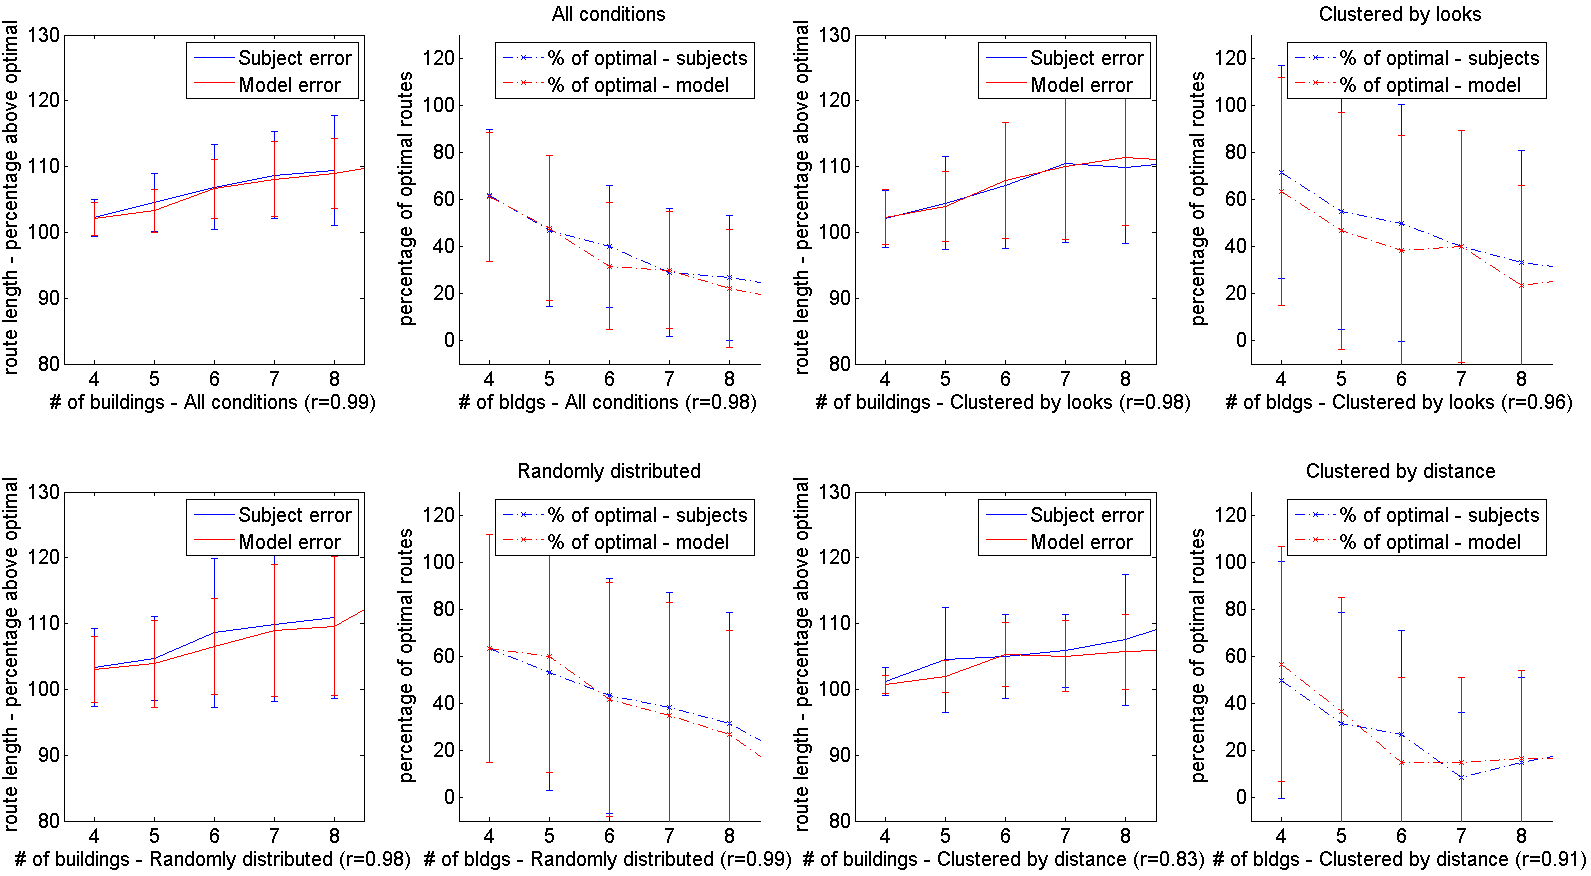
\includegraphics[width=\textwidth]{img/tsperrors2}
	\end{center}
	\caption[Human performance in virtual reality, compared to gradient-based planning]{
		{\bf Human performance in virtual reality, compared to gradient-based planning} on a flat grid of place nodes. 
	}
	\label{tsp}
\end{figure}

\begin{figure}[!ht]
	\begin{center}
		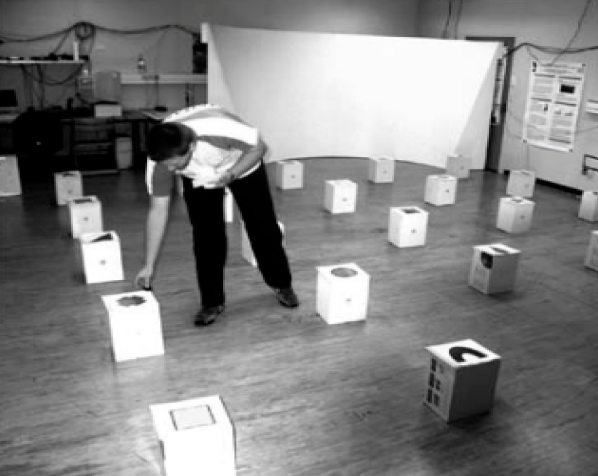
\includegraphics[width=0.49\textwidth]{img/wienerexp}
		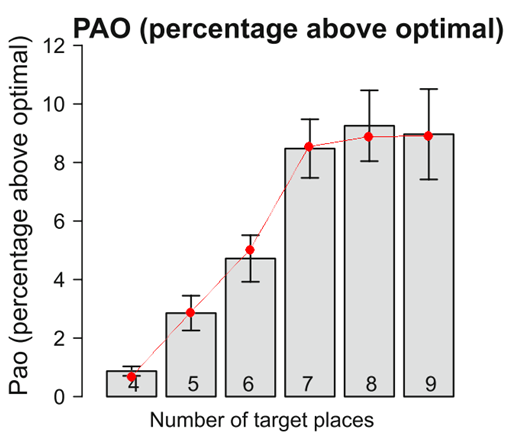
\includegraphics[width=0.49\textwidth]{img/wieneretal2009_spatial_tsp_comparison.png}
	\end{center}
	\caption[Human performance in a real-world experiment]{
		{\bf Human performance in a real-world experiment \citep{Wiener2009}, compared to gradient-based planning,} on a hierarchical grid of place nodes. Figures modified from \citep{Wiener2009} with permission.
	}
	\label{tsp2}
\end{figure}


%An appendix is just like any other chapter, except that it comes after
%the appendix command in the master file.
%
%One use of an appendix is to include an example of input to the system
%and the corresponding output.
%
%One way to do this is to include, unformatted, an existing input file. 
%You can do this using \verb=\verbatiminput=. In this appendix we
%include a copy of the C file \textsf{hello.c} and its output file
%\textsf{hello.out}. If you use this facility you should make sure that
%the file which you input does not contain \texttt{TAB} characters,
%since \LaTeX\ treats each \texttt{TAB} as a single space; you can use
%the Unix command \texttt{expand} (see manual page) to expand tabs into
%the appropriate number of spaces. 
%
%\section{Example input and output}
%\label{sec:inp-eg}
%\subsection{Input}
%\label{sec:input}
%(Actually, this isn't input, it's the source code, but it will do as
%an example)
%
%\verbatiminput{hello.c}
%
%\subsection{Output}
%\label{sec:output}
%
%\verbatiminput{hello.out}
%\subsection{Another way to include code}
%You can also use the capabilities of the \texttt{listings} package to
%include sections of code, it does some keyword highlighting.
%
%\lstinputlisting[language=C]{hello.c}


\begin{thebibliography}{2}
	\expandafter\ifx\csname natexlab\endcsname\relax\def\natexlab#1{#1}\fi
	\providecommand{\url}[1]{\texttt{#1}}
	\providecommand{\href}[2]{#2}
	\providecommand{\path}[1]{#1}
	\providecommand{\DOIprefix}{doi:}
	\providecommand{\ArXivprefix}{arXiv:}
	\providecommand{\URLprefix}{URL: }
	\providecommand{\Pubmedprefix}{pmid:}
	\providecommand{\doi}[1]{\href{http://dx.doi.org/#1}{\path{#1}}}
	\providecommand{\Pubmed}[1]{\href{pmid:#1}{\path{#1}}}
	\providecommand{\bibinfo}[2]{#2}
	\ifx\xfnm\relax \def\xfnm[#1]{\unskip,\space#1}\fi
	%Type = Inproceedings
	\bibitem[{Madl et~al.(2013)Madl, Franklin, Chen \& Trappl}]{madl2013spatial}
	\bibinfo{author}{Madl, T.}, \bibinfo{author}{Franklin, S.},
	\bibinfo{author}{Chen, K.}, \& \bibinfo{author}{Trappl, R.}
	(\bibinfo{year}{2013}).
	\newblock \bibinfo{title}{Spatial working memory in the lida cognitive
		architecture}.
	\newblock In {\it \bibinfo{booktitle}{Proc. international conference on
			cognitive modelling}\/}.
	%Type = Article
	\bibitem[{Wiener et~al.(2009)Wiener, Ehbauer \& Mallot}]{Wiener2009}
	\bibinfo{author}{Wiener, J.~M.}, \bibinfo{author}{Ehbauer, N.~N.}, \&
	\bibinfo{author}{Mallot, H.~a.} (\bibinfo{year}{2009}).
	\newblock \bibinfo{title}{{Planning paths to multiple targets: memory
			involvement and planning heuristics in spatial problem solving.}}
	\newblock {\it \bibinfo{journal}{Psychological research}\/},  {\it
		\bibinfo{volume}{73}\/}, \bibinfo{pages}{644--58}.
	\DOIprefix\doi{10.1007/s00426-008-0181-3}.
	
\end{thebibliography}




%\bibliography{lidaspm}

%\end{document}